\chapter{Aritmética de Máquina}
\section{Sistema de Numeração e Mudança de Base}
No Ocidente utilizamos um sistema de numeração decimal para representar números. Esse é um sistema de numeração posicional onde a posição do dígito indica a potência de $10$ que o dígito está representando.

\begin{ex}
  Observe o número 293 decomposto em centenas, dezenas e unidades:
  \begin{eqnarray*}
    293&=&2\ \hbox{centenas}+9\ \hbox{dezenas}+3\ \hbox{unidades}\\
    &=&2\cdot 10^2+9\cdot 10^1+3\cdot 10^0.
  \end{eqnarray*}
  Ou seja, as centenas, dezenas e unidades são potências de 10.
\end{ex}

\begin{defn}(Sistema de numeração de base $b$)
Dado um número natural $b>1$ e  a coleção de símbolos $\{\text{``.''}, - ,0, 1, \cdots, b-1\}$, a sequência de dígitos
$$
(d_nd_{n-1}\cdots d_1d_0,d_{-1}d_{-2}\cdots)_b
$$
representa o número positivo
$$
d_nb^n+d_{n-1}b^{n-1}+\cdots d_0b^0+d_{-1}b^{-1}+\cdots
$$
Para representar números negativos usamos o sinal ``-'' na frente do numeral.
\end{defn}

\begin{obs}($b\geq 10$)

\begin{itemize}
\item Quando o índice $b$ não aparece no numeral, entendemos $b=10$.
\item Quando b>10, usamos as letras $A$, $B$, $C$, etc, para completar os símbolos: $A=10$, $B=11$, $C=12$, $D=13$, $E=14$, $F=15$, etc.
\end{itemize}
\end{obs}

% \begin{ex}
% $$
% (301,2)_{4}=3\cdot 4^2+0\cdot 4^1+1\cdot 4^0+2\cdot 4^{-1}=49,5
% $$
% \end{ex}

\begin{ex} (Sistema Binário)
Nesse sistema um \textit{bit} pode assumir dois valores distintos entre os símbolos $0$ ou $1$. Por exemplo,
\begin{eqnarray*}
(1001.101)_{2}&=&1\cdot 2^3 +0\cdot 2^2 +0\cdot 2^1 +1\cdot 2^0  +1\cdot 2^{-1} +0\cdot 2^{-2} +1\cdot 2^{-3} \\ &=&8+0+0+1+ 0,5+0+0,125=(9,625)_{10}
\end{eqnarray*}
\end{ex}

\begin{ex} (Sistema Octal)
Nesse sistema a base é $b=8$ e utilizamos os símbolos em $\{0, 1, 2, 3, 4, 5, 6, 7\}$. Por exemplo,
\begin{eqnarray*}
(1357,24)_{8}&=&1\cdot 8^3+3\cdot 8^2+5\cdot 8^1+7\cdot 8^{0}+2\cdot 8^{-1}+4\cdot 8^{-2}\\&=&512+192+40+7+0,25+0,0625=(751,3125)_{10}
\end{eqnarray*}
\end{ex}


\begin{ex} (Sistema de numeração hexadecimal) Tomando $b=16$  o conjunto de símbolos necessários é  $S=\{0,\ 1,\ 2,\ 3,\ 4,\ 5,\ 6,\ 7,\ 8,\ 9,\ A,\ B,\ C,\ D,\ E,\ F\}$. O número $(E2AC)_{16}$ nesse sistema é
\begin{eqnarray*}
(E2AC)_{16}&=&14\cdot 16^3+2\cdot 16^2+10\cdot 16^1+12\cdot 16^{0}\\&=&57344+512+160+12=(58028)_{10}
\end{eqnarray*}
\end{ex}

\begin{prob}Escreva os números abaixo na base decimal
\begin{description}
\item[a)] $(25,13)_8$
\item[b)] $(101,1)_2$
\item[c)] $(12F,4)_{16}$
\item[d)] $(11,2)_{3}$
\end{description}
\end{prob}

Agora desejamos fazer o processo inverso, ou seja, escrever um número decimal dado numa base $b$. Consideramos um número decimal $X_{10}$ representado na base $b$
$$
X_{10}=(d_nd_{n-1}\cdots d_0,d_{-1}\cdots)_{b}=d_n\cdot b^{n}+d_{n-1}\cdot b^{n-1}+\cdots +d_1\cdot b^1+d_0\cdot b^0+d_{-1}\cdot b^{-1}+d_{-2}\cdot b^{-2}+\cdots
$$
e separamos em parte inteira e parte fracionária, $X=X^{i}+X^{f}$, onde
$$
X^{i}=d_n\cdot b^{n}+ \cdots+d_{n-1}b^{n-1} \cdot  +d_1\cdot b^1 +d_0\cdot b^0 \qquad \hbox{e}\qquad X^{f}
= \frac{d_{-1}}{b^1}+\frac{d_{-2}}{b^{2}}+\cdots
$$

Nosso objetivo é encontrar os símbolos $\{d_n, d_{n-1}, ...\}$. Primeiro tratamos a parte inteira $X^{i}$ olhando a divisão por $b$
$$
\frac{X^{i}}{b}=   \frac{d_0}{b}+d_1+d_2 b^1\cdots+d_{n-1}\cdot b^{n-2} +d_n\cdot b^{n-1}.
$$
Observe que $d_0$ é o resto da divisão de $X^i$ por $b$, pois $d_1+d_2 b^1\cdots+d_{n-1}\cdot b^{n-2} +d_n\cdot b^{n-1}$ é inteiro e $\frac{d_0}{b}$ é uma fração (lembramos que $d_0<b$). Da mesma forma, o resto da divisão de $d_1+d_2 b^1\cdots+d_{n-1}\cdot b^{n-2} +d_n\cdot b^{n-1}$ por $b$ é $d_1$. Repetimos o processo até encontrar os símbolos $d_0$, $d_1$, $d_2$,....
\begin{ex}Escrever o número 125 na base $6$.

Para encontrar $d_0$, dividimos $125$ por 6
$$
\begin{array}{l}
125 \ \ \ |\! \underline{\ \ 6\ \ } \\
\underline{\ 7 }\ \ \ \ \ \ \ 20\\
\ 05\\
\ \underline{00}\\
\ \ 5
\end{array}
$$
e encontramos $d_0=5$. Dividindo o quociente por $6$ para encontrar $d_1$
$$
\begin{array}{l}
20 \ \ \ |\! \underline{\ \ 6\ \ } \\
\underline{18 }\ \ \ \ \ 3\\
\ 2
\end{array}
$$
e obtemos $d_1=2$. Observe que o quociente agora é menor que $6$, ou seja, uma divisão por $6$ obviamente tem resto igual a $3$. Portanto
$$
125=(325)_6
$$
\end{ex}


Para encontrar os símbolos $d_{-1}$, $d_{-2}$, etc, olhamos a parte fracionária de $X$ quando multiplicamos por $b$:
$$
bX^{f}=d_{-1}+\frac{d_{-2}}{b}+\frac{d_{-3}}{b^2}+\cdots.
$$
Observe que a parte inteira desse produto é $d_{-1}$ e $\frac{d_{-2}}{b}+\frac{d_{-3}}{b^2}+\cdots$ é a parte fracionária. Quando multiplicamos $\frac{d_{-2}}{b}+\frac{d_{-3}}{b^2}+\cdots$ por $b$ novamente, encontramos $d_{-2}$. Repetimos o processo até encontrar todos os símbolos.
\begin{ex}Escrever o número $125,58\overline{3}$ na base $6$.

Do exemplo anterior temos que $125=(325)_6$. Portanto multiplicamos a parte fracionária $0,58\overline{3}$ por $6$
$$
\begin{array}{l}
0,58\overline{3}\\
\underline{\times\ 6}\\
3,49 \overline{9}
\end{array}
$$
e obtemos $d_{-1}=3$. Agora, multiplicamos $0,49\overline{9}=0,5$ por $6$
$$
\begin{array}{l}
0,5\\
\underline{\times\ 6}\\
3,0
\end{array}
$$
e obtemos $d_{-2}=3$. Portanto
$$
125,58\overline{3}=(325,33)_6
$$
\end{ex}
\begin{prob} Escreva cada número decimal na base $b$

\begin{description}
\item[a)] $7,\overline{6}$ na base $b=5$
\item[b)] $29,1\overline{6}$ na base $b=6$
\end{description}
\end{prob}

Um maneira de converter um número dado numa base $g$ para uma base $b$ é fazer em duas partes: primeiro converter o número dado na base $g$ para base decimal e depois converter para a base $b$.

\begin{prob} Escreva cada número dado para a base $b$.

\begin{description}
\item[a)] $(45,1)_8$ para a base $b=2$
\item[b)] $(21,2)_8$ para a base $b=16$
\item[c)] $(1001,101)_2$ para a base $b=8$
\item[d)] $(1001,101)_2$ para a base $b=16$
\end{description}
\end{prob}








\section{Aritmética de Máquina}
Os computadores, em geral, usam uma base binária para representar os números, onde as posições, chamadas de bits, assume as condições ``verdadeiro'' ou ``falso'', ou seja, $0$ ou $1$. Cada computador tem um número de bits fixo e, portanto, representa uma quantidade finita de números. Os demais números são tomados por proximidade àqueles conhecidos, gerando erros de arredondamento. Por exemplo, em aritmética de computador, o número $2$ tem representação exata, logo $2^2=4$, mas $\sqrt{3}$ não tem representação finita, logo $(\sqrt{3})^2\neq 3$.



%\subsection{Sistema de ponto fixo}
\subsection{Representação de números inteiros}

Tipicamente um número inteiro é armazenado num computador como uma sequência de dígitos binários de comprimento fixo denominado registro.

\subsubsection{Representação sem sinal}
Um registro com $n$ bits da forma
$$
\begin{array}{|c|c|c|c|c|} \hline
d_{n-1}&d_{n-2}&\cdots&d_1&d_0\\\hline
\end{array}
$$
representa o número $(d_{n-1}d_{n-2}...d_1d_0)_2$. Assim é possível representar números inteiros entre
$$
\begin{array}{cl}
  (111...111)_2 & = 2^{n-1}+2^{n-2}+\cdots+2^1+2^0=2^n-1.\\
    \vdots      & = \\
  (000...000)_2 & = (0)_{10} \\
\end{array}
$$


\subsubsection{Representação com bit de sinal}
O bit mais significativo (o primeiro à esquerda) representa o sinal: 0 positivo e 1 negativo. Um registro com $n$ bits da forma
$$
\begin{array}{|c|c|c|c|c|} \hline
s&d_{n-2}&\cdots&d_1&d_0\\\hline
\end{array}
$$
representa o número $(-1)^s(d_{n-1}d_{n-2}...d_1d_0)_2$. Assim é possível representar números inteiros entre $-2^{n-2}$ e $2^{n-2}$, com duas representações para o zero: $(1000...000)_2$ e $(00000...000)_2$.
\begin{ex}
Em um registro com $32$ bits, teremos os números
$$
\begin{array}{cl}
 (11111111)_2 &= -(2^{6}+\cdots+2+1)=-127_{10}\\
     \vdots    &=  \\
 (10000001)_2 &= -1_{10} \\
 (10000000)_2 &= -0_{10} \\
 (01111111)_2 &= 2^6+\cdots+2+1=127_{10} \\
     \vdots    &=  \\
 (00000010)_2 &= 2_{10} \\
 (00000001)_2 &= 1_{10} \\
 (00000000)_2 &= 0_{10} \\
\end{array}
$$
\end{ex}

%\subsubsection{Representação complemento de um}

\subsubsection{Representação complemento de dois}
O bit mais significativo (o primeiro à esquerda) representa o termo $-2^{n-1}$ se $d_{n-1}=1$.  Um registro com $n$ bits da forma
$$
\begin{array}{|c|c|c|c|c|} \hline
d_{n-1}&d_{n-2}&\cdots&d_1&d_0\\\hline
\end{array}
$$
representa o número $-d_{n-1}2^{n-1}+(d_{n-2}...d_1d_0)_2$. 

Note que todo registro começando com $1$ será um número negativo.

\begin{ex}
 O registro com $8$ bits $[01000011]$ representa o número
 $-0(2^7)+(1000011)_2=64+2+1=67_{10}$.

 O registro com $8$ bits $[10111101]$ representa o número
 $-1(2^7)+(0111101)_2=-128+ 32+16+8+4+1=-67_{10}$.

 Note que podemos obter a representação de $-67_{10}$ invertendo os dígitos de $67_{10}$ em binário e somando 1.
\end{ex}

\begin{ex}
Em um registro com $8$ bits, teremos os números
$$
\begin{array}{cl}
 (11111111)_2 &= -2^7+2^{6}+\cdots+2+1=-1_{10}\\
     \vdots   &=  \\
 (10000001)_2 &= -2^7+1 = -127_{10} \\
 (10000000)_2 &= -2^7   = -128_{10} \\
 (01111111)_2 &= 2^6+\cdots+2+1=127_{10} \\
     \vdots    &=  \\
 (00000010)_2 &= 2_{10} \\
 (00000001)_2 &= 1_{10} \\
 (00000000)_2 &= 0_{10} \\
\end{array}
$$
\end{ex}





\subsection{Sistema de ponto fixo}
O sistema de ponto fixo representa as partes inteira e fracionária do número com uma quantidade fixas de dígitos. 

\begin{ex} Um computador de 32 bits que usa o sistema de ponto fixo, o registro
$$
\begin{array}{|c|c|c|c|c|c|} \hline
d_{31}&d_{30}&d_{29}&\cdots&d_1&d_0\\\hline
\end{array}
$$
pode representar o número
\begin{itemize}
\item $(-1)^{d_{31}}(d_{30}d_{29}\cdots d_{17}d_{16},d_{15}d_{14}\cdots d_1d_0)_2$
se o sinal for representado por um dígito. Observe que nesse caso o zero possui duas representações possíveis: 
$$
10000000000000000000000000000000\qquad \hbox{e}\qquad 00000000000000000000000000000000
$$
\item $(d_{30}d_{29}\cdots d_{17}d_{16})_2-d_{31}(2^{15}-2^{-16})+(0,d_{15}d_{14}\cdots d_1d_0)_2$
se o sinal do número estiver representado por uma implementação em complemento de um. Observe que o zero também possui duas representações possíveis: 
$$
11111111111111111111111111111111\qquad \hbox{e}\qquad 00000000000000000000000000000000
$$
\item $(d_{30}d_{29}\cdots d_{17}d_{16})_2-d_{31}2^{15}+(0,d_{15}d_{14}\cdots d_1d_0)_2$
se o sinal do número estiver representado por uma implementação em complemento de dois. Nesse caso o zero é unicamente representado por
$$
00000000000000000000000000000000
$$
\end{itemize}



Observe que 16 dígitos são para representar a parte fracionária, 15 são para representar a parte inteira e um dígito, o $d_{31}$, está relacionado ao sinal do número. 
\end{ex}

\subsection{Sistema de ponto flutuante}
O sistema de ponto flutuante não possui quatidade fixa de dígitos para as partes inteira e fracionária do número. 

\begin{ex} Um computador de 64 bits que usa o sistema de ponto flutuante com um dígito para o sinal, o registro
$$
\begin{array}{|c|c|c|c|c|c|c|c|c|c|}
\hline
s&c_{10}&c_{9}&\cdots&c_{0}&m_{-1}&m_{-2}&\cdots &m_{-50}&m_{-51}\\
\hline
\end{array}
$$
representa o número
$$
(-1)^{s}2^{c-1023}(1+m),
$$
onde
$$
c=c_{10}2^{10}+c_92^9+\cdots+c_12^1+c_02^0\qquad\hbox{e}\qquad m=m_{-1}2^{-1}+m_{-2}2^{-2}+\cdots+m_{-50}2^{-50}+m_{-51}2^{-51}.
$$
Os dígitos $c_{10}, c_9\, \cdots, c_0\ $ compõem a característica e $m_{-1}, m_{-2}\, \cdots, m_{-51}\ $ compõem a mantissa. Por exemplo, o número
$$
0\ 1 0 0 0 0 0 0 0 0 0 0 \ 1 0 0 0 0 0 0 0 0 0 0 0 0 0 0 0 0 0 0 0 0 0 0 0 0 0 0 0 0 0 0 0 0 0 0 0 0 0 0 0 0 0 0 0 0 0 0 0 0 0 0 0
$$
representa o número
$$
(-1)^0 2^{1024-1023}(1+2^{-1})=3
$$
O menor número positivo nesse sistema acontece quando $s=0$, $c=1$ e $m=0$, ou seja,
$$
2^{-1022}(1+0)\approx 0,2225\times 10^{-307}.
$$
O maior número acontece quando $s=0$, $c=2046$ e $f=1-2^{-52}$, ou seja,
$$
2^{1023}(2-2^{-52})\approx 0,17977\times 10^{309}.
$$
\end{ex}
Um número muito pequeno (underflow) geralmente é aproximado por zero e um número muito grande (overflow) geralmente faz o cálculo parar. Os demais números são aproximados pelo mais próximo, gerando os erros de arredondamento. Em geral, um sistema de ponto flutuante com $m+n+1$ bits representa o número
$$
\pm 0,d_{-1}d_{-2}\cdots d_{-n} b^e,
$$
onde $b$ é a base, $1<d_{-1}\leq b-1$ e $0\leq d_{-i}\leq b-1$, $i=2,...,n$, formam o significado, $e$ é o expoente formado por $m$ bits e um bit representa o sinal. Nesse caso dizemos que o número possui $n$ {\bf dígitos significativos}. Por simplicidade, a partir daqui nós adotaremos $b=10$.
\begin{ex}Represente os números $0,00\overline{51}$ e $1205,41\overline{54}$ em um sistema de ponto fixo de 4 dígitos para a parte inteira e 4 dígitos para a parte fracionária. Depois represente os mesmos números num sistema de ponto flutuante com 8 dígitos significativos.

No sistema de ponto fixo os números são: $0,0051$ e $1205,4154$.

No sistema de ponto flutuante temos: $0,51515151\cdot 10^{-2}$ e $0,12054154 \cdot 10^{4}$.
\end{ex}


\section{Origem e Definição de Erros}
Quando fazemos aproximações numéricas, os erros são gerados de várias formas, sendo as principais delas as seguintes:
\begin{enumerate}
 \item Dados de entrada: equipamentos de medição possuem precisão finita, acarretando erros nas medidas físicas.
 \item Erros de Truncamento: ocorrem quando aproximamos um procedimento formado por uma sequência infinita de passos através de um outro procedimento finito. Por exemplo, a definição de integral é dada por uma soma infinita e, como veremos na terceira área, aproximaremos-a por um soma finita. Esse é um assunto que discutiremos várias vezes no curso, pois o tratamento do erro de truncamento é feito para cada método numérico.
 \item Erros de Arredondamento: são aqueles relacionados com as limitações que existem na forma representar números de máquina. Sobre esse tópico dedicamos a subseção (\ref{arredondamento_sec}).
\end{enumerate}


\begin{defn} Seja $x$ um número real e $\overline{x}$ sua aproximação, então $|x-\overline{x}|$ é o erro absoluto e $\dfrac{|x-\overline{x}|}{|x|}$ é o erro relativo. Observe que o erro relativo é adimensional e, por isso, faz sentido escrever em porcentagem.
\end{defn}
\begin{ex}
Se $x=\frac{1}{3}$ e $\overline{x}=0,333$, então o erro absoluto é
$$
|x-\overline{x}|=|0,\overline{3}-0,333|=0,000\overline{3}=0,\overline{3}\cdot 10^{-3}
$$
e o erro relativo é
$$
\frac{|x-\overline{x}|}{|x|}=\frac{0,\overline{3}\cdot 10^{-3}}{0,\overline{3}}=10^{-3}=0,1\%
$$
\end{ex}

\begin{ex}
Observe os erros absolutos e relativos em cada caso
$$
\begin{array}{|c|c|c|}
\hline
&\hbox{erro absoluto}&\hbox{erro relativo}\\
\hline
x=0,\overline{3}\cdot 10^{-2}\ \hbox{e}\ \overline{x}=0,3\cdot 10^{-2}&0,\overline{3}\cdot 10^{-3}&\frac{0,\overline{3}\cdot 10^{-3}}{0,\overline{3}\cdot 10^{-2}}=10^{-1}=10\%\\
\hline
x=0,\overline{3}\ \hbox{e}\ \overline{x}=0,3&0,\overline{3}\cdot 10^{-1}&\frac{0,\overline{3}\cdot 10^{-1}}{0,\overline{3}}=10^{-1}=10\%\\
\hline
x=0,\overline{3}\cdot 10^{2}\ \hbox{e}\ \overline{x}=0,3\cdot 10^{2}&0,\overline{3}\cdot 10^{1}&\frac{0,\overline{3}\cdot 10^{1}}{0,\overline{3}\cdot 10^{2}}=10^{-1}=10\%\\
\hline
\end{array}
$$
\end{ex}

\begin{prob}Calcule os erros absoluto e relativo das aproximações $\overline{x}$ para $x$
\begin{description}
\item[a)] $x=\pi=3,14159265358979\cdots$ e $\overline{x}=3,141$
\item[b)] $x=1,00001$ e $\overline{x}=1$
\item[c)] $x=100001$ e $\overline{x}=100000$
\end{description}
\end{prob}

\begin{defn}
A aproximação $\overline{x}$ de um número $x$ da forma $\overline{x}=\pm 0,d_{-1}d_{-2}\cdots d_{s}\cdots d_n\cdot 10^m$ possui $s$ dígitos significativos corretos se o erro absoluto $|x-\overline{x}|$ satisfazer\footnote{Observação: Não existe uma definição única na literatura para o conceito de dígitos significativos corretos, embora não precisamente equivalentes, transmitem a mesmo conceito.}
$$
|x-\overline{x}|\leq 0,5\cdot 10^{m-s}
$$
\end{defn}
\begin{ex}
\begin{description}
\item[a)] Considere $x=0,\overline{3}$, $\overline{x}=0,333$ e o erro absoluto $\delta=|x-\overline{x}|=0,\overline{3}\cdot 10^{-3}=0,\overline{3}\cdot 10^{0-3}$. Essa aproximação tem 3 dígitos significativos corretos.
\item[b)] Agora, considere $x=10,00\overline{1}=0,1000\overline{1}\cdot 10^{2}$, $\overline{x}=9,99933=0,999933\cdot 10^1$ e o erro absoluto $\delta=|x-\overline{x}|=0,178\overline{1}\cdot 10^{-2}=0,178\overline{1}\cdot 10^{1-3}$. Essa aproximação possui todos os dígitos diferentes se comparamos um a um, mas tem 3 dígitos significativos corretos.
\end{description}
\end{ex}
\begin{prob}
Verifique quantos são os dígitos significativos corretos em cada aproximação $\overline{x}$ para $x$.
\begin{description}
\item[a)] $x=2,5834$ e $\overline{x}=2,6$
\item[b)] $x=100$ e $\overline{x}=99$
\end{description}
\end{prob}



\subsection{Erros de Arredondamento}{\label{arredondamento_sec}}
Os erros de arredondamento são aqueles gerados quando aproximamos um número real por um número com representação finita.

\begin{ex}
O número $\frac{1}{3}=0,\overline{3}$ possui um representação infinita tanto na base decimal quanto na base binária. Logo, quando representamos ele no computador gera um erro de arredondamento que denotaremos por $\epsilon$. Agora considere a seguinte sequência:
$$
\left\{\begin{array}{l}
x_0=\frac{1}{3}\\
x_{n+1}=4x_n-1,\qquad n\in\mathbb{N}
\end{array}\right..
$$
Observe que $x_0=\frac{1}{3}$, $x_1=4\cdot \frac{1}{3}-1=\frac{1}{3}$, $x_2=\frac{1}{3}$, ou seja, temos uma sequência constante igual a $\frac{1}{3}$. Se calcularmos no computador essa sequência, temos que incluir os erros de arredondamento, ou seja,
\begin{eqnarray*}
\tilde{x}_0&=&\frac{1}{3}+\epsilon\\
\tilde{x}_1&=&4x_0-1=4\left(\frac{1}{3}+\epsilon\right)-1=\frac{1}{3}+4\epsilon\\
\tilde{x}_2&=&4x_1-1=4\left(\frac{1}{3}+4\epsilon\right)-1=\frac{1}{3}+4^2\epsilon\\
&\vdots&\\
\tilde{x}_n&=&\frac{1}{3}+4^n\epsilon
\end{eqnarray*}
Portanto o limite da sequência diverge,
$$
\lim_{x\to\infty}|\tilde{x}_n|=\infty
$$
Faça o teste no scilab, colocando $x=1/3$ e calculando $x=4*x-1$ algumas dezenas de vezes.
\end{ex}

Para aproximar o número $\pm 0,d_{-1}d_{-2}d_{-3}d_{-4}\cdots 10^e$ com $k$ dígitos significativos existem várias regras, sendo as duas principais as seguintes:
\begin{enumerate}
\item Truncamento aproxima esse número por
$$
\pm 0,d_{-1}d_{-2}d_{-1}d_{-4}\cdots d_{-k} 10^e
$$
simplesmente descartando os dígitos além de $d_{-k}$.
\item Arredondamento aproxima esse número por
$$
\pm 0,g_{-1}g_{-2}g_{-1}g_{-4}\cdots g_{-k} 10^{\tilde{e}}
$$
que é um truncamento do número
$$
\pm 0,d_{-1}d_{-2}d_{-1}d_{-4}\cdots d_{-k}d_{-k-1} 10^e \pm 0,000\cdots 5\cdot 10^e,
$$
onde o segunda número possui $k$ zeros, ou seja, $k+1$ dígitos significativos. Observe que um arredondamento pode mudar todos os dígitos e o expoente.
\end{enumerate}

\begin{ex} Represente os números $0,567$; $0,233$; $-0,6785$ e $\pi =3,14159265...=0,314159265...\times 10^1$ com dois dígitos significativos por truncamento e arredondamento.

Truncamento: $0,56$; $0,23$; $-0,67$ e $\pi =0,31\times 10^1=3,1$

Arredondamento: $0,57$; $0,23$; $-0,68$ e $\pi =0,31\times 10^1=3,1$
\end{ex}

\begin{prob}  Represente os números $3276$; $42,55$ e $0,00003331$ com três dígitos significativos por truncamento e arredondamento.
\end{prob}

\begin{prob} Resolva a equação $0,1x-0,01=12$ usando arredondamento com três dígitos significativos em cada passo e compare com o resultado analítico
\end{prob}



\section{Propagação de Erros}

Dado uma função diferenciável $f$, considere $\overline{x}$ uma aproximação para $x$ e $f(\overline{x})$ uma aproximação para $f(x)$. Sabendo o erro $\delta_x=|x-\overline{x}|$, queremos estimar o erro $\delta_f=|f(x)-f(\overline{x})|$. Pelo teorema do valor médio, existe $\epsilon$ contido no intervalo aberto formado por $x$ e $\overline{x}$ tal que
$$
f(x)-f(\overline{x})=f'(\epsilon)(x-\overline{x}).
$$
Como não conhecemos o valor de $\epsilon$, supomos que a derivada $f'(\epsilon)$ é limitada por $M$ ($|f'(\epsilon)|\leq M$) no intervalo fechado formado por $x$ e $\overline{x}$ e obtemos
$$
|f(x)-f(\overline{x})|\leq M|x-\overline{x}|.
$$
Se $f'(x)$ não varia muito rápido nesse intervalo e supondo $\delta_x$ pequeno, aproximamos $M\approx |f'(\overline{x})|$ e temos:
$$
|f(x)-f(\overline{x})|\approx |f'(\overline{x})||x-\overline{x}|,
$$
ou
$$
\delta_f\approx |f'(\overline{x})|\delta_x.
$$
De modo geral, quando $f$ depende de várias variáveis, a seguinte estimativa vale:
$$
\delta_f=|f(x_1,x_2,...,x_n)-f(\overline{x}_1, \overline{x}_2,...,\overline{x}_n)|\approx \sum_{i=1}^n\left|\frac{\partial f}{\partial x_i}(\overline{x}_1, \overline{x}_2,...,\overline{x}_n)\right|\delta_{x_i}
$$
\begin{ex}
Considere um triângulo retângulo onde a hipotenusa e um dos catetos são conhecidos a menos e um erro: hipotenusa $a=3\pm 0,01$ metros e cateto $b=2\pm 0,01$ metros. Calcule o erro absoluto ao calcular a área dessa triângulo.

Primeiro vamos encontrar a expressão para a área em função da hipotenusa $a$ e um cateto $b$. A tamanho de segundo cateto $c$ é dado pelo teorema de pitágoras, $a^2=b^2+c^2$, ou seja, $c=\sqrt{a^2-b^2}$. Portanto a área é $$
A=\frac{bc}{2}=\frac{b\sqrt{a^2-b^2}}{2}.
$$
Agora calculamos as derivadas
$$
\frac{\partial A}{\partial a}=\frac{ab}{2\sqrt{a^2-b^2}},
$$
$$
\frac{\partial A}{\partial b}=\frac{\sqrt{a^2-b^2}}{2}-\frac{b^2}{2\sqrt{a^2-b^2}},
$$
e substituindo na estimativa para o erro $\delta_A$ em termos de $\delta_a=0,01$ e $\delta_b=0,01$:
\begin{eqnarray*}
\delta_A&\approx & \left|\frac{\partial A}{\partial a}\right|\delta_a+\left|\frac{\partial A}{\partial b}\right|\delta_b\\
&\approx &\frac{3\sqrt{5}}{5}\cdot 0,01+\frac{\sqrt{5}}{10}\cdot 0,01=0.01565247584
\end{eqnarray*}
Em termos do erro relativo temos erro na hipotenusa de $\frac{0,01}{3}\approx 0,333\%$, erro no cateto de $\frac{0,01}{2}= 0,5\%$ e erro na área de
$$
\frac{0.01565247584}{\frac{2\sqrt{3^2-2^2}}{2}}=0,7\%
$$
\end{ex}

\begin{ex} Calcule o erro relativo ao medir $f(x,y)=\frac{x^2+1}{x^2}e^{2y}$ sabendo que $x\approx 3$ é conhecido com $10\%$ de erro e $y\approx 2$ é conhecido com $3\%$ de erro.

Calculamos as derivadas parciais de $f$:
$$
\frac{\partial f}{\partial x}=\frac{2x^3-(2x^3+2x)}{x^4}e^{2y}=-\frac{2e^{2y}}{x^3}
$$
e
$$
\frac{\partial f}{\partial y}=2\frac{x^2+1}{x^2}e^{2y}
$$
Calculamos o erro absoluto em termos do erro relativo:
$$
\frac{\delta_x}{|x|}=0,1\Rightarrow \delta_x= 3\cdot 0,1=0,3
$$
$$
\frac{\delta_y}{|y|}=0,03\Rightarrow \delta_y= 2\cdot 0,03=0,06
$$
Aplicando a expressão para estimar o erro em $f$ temos
\begin{eqnarray*}
\delta_f &\leq& \left|\frac{\partial f}{\partial x}\right|\delta_x+\left|\frac{\partial f}{\partial y}\right|\delta_y\\
&\leq& \frac{2e^{4}}{27}\cdot 0,3+2\frac{9+1}{9}e^{4}\cdot 0,06=8,493045557
\end{eqnarray*}
Portanto, o erro relativo ao calcular $f$ é estimado por
$$
\frac{\delta f}{|f|}=\frac{8,493045557}{\frac{9+1}{9}e^{4}}=14\%
$$
\end{ex}
\begin{ex} No exemplo anterior, reduza o erro retivo em $x$ pela metade e calcule o erro relativo em $f$. Depois, repita o processo reduzindo o erro relativo em $y$ pela metade.

Na primeira situação temos $x=3$ com erro relativo de $5\%$ e $\delta_x=0,05\cdot 3=0,15$. Calculamos $\delta_f=7.886399450$ e o erro relativo em $f$ de $13\%$. Na segunda situação, temos $y=2$ com erro de $1,5\%$ e $\delta_y=2\cdot 0,015=0,03$. Calculamos $\delta_f=4.853168892$ e o erro relativo em $f$ de $8\%$. Observe que mesma o erro relativo em $x$ sendo maior, o erro em $y$ é mais significante na função.
\end{ex}

\begin{prob} A corrente $I$ em ampères e a tensão $V$ em volts em uma lâmpada se relacionam conforme a seguinte expressão:
$$I=\left(\frac{V}{V_0}\right)^\alpha$$
Onde $\alpha$ é um número entre 0 e 1 e $V_0$ é tensão nominal em volts. Sabendo que $V_0=220\pm 3\%$ e $\alpha=.8\pm 4\%$
Calcule a corrente e o erro relativo associado quando a tensão vale $220\pm 1\%$.

{\bf Dica:} lembre que $x^\alpha=e^{\alpha \ln(x)}$
\end{prob}


\section{Cancelamento Catastrófico}
Operações aritméticas entre números com representação finita pode fazer com que o resultado seja dominado pelos erros de arredondamento. Em geral, esse efeito, denominado cancelamento catastrófico, acontece quando fazemos a diferença de números muito próximos entre si.

\begin{ex}Efetue a operação
$$
0,987624687925-0,987624=0,687925\times 10^{-6}
$$
usando arredontamento com seis dígitos significativos e observe a diferença se comparado com resultado sem arredondamento.

Os números arredondados com seis dígitos para a mantissa resultam na seguinte diferença
$$
0,987625-0,987624=0,100000\times 10^{-5}
$$
Observe que os erros relativos entre os números exatos e aproximados no lado esquerdo é bem pequeno,
$$
\frac{|0,987624687925-0,987625|}{|0,987624687925|}=0,00003159\%\qquad\hbox{e}\qquad \frac{0,987624-0,987624}{0,987624}=0\%,
$$
enquanto no lado direito o erro relativo é enorme,
$$
\frac{|0,100000\times 10^{-5}-0,687925\times 10^{-6}|}{0,687925\times 10^{-6}}=45,36\%
$$

\end{ex}

\begin{ex} Encontre as raízes da equação de segundo grau
$$
x^2+300x-0,014=0
$$
usando seis dígitos significativos.

Usando a fórmula de Báskara com $a=0,100000\times 10^1$, $b=0,300000\times 10^3$ e $c=0,140000\times 10^{-1}$, temos
\begin{eqnarray*}
\Delta&=&0,300000\times 10^3\times 0,300000\times 10^3 +0,400000\times 10^1\times 0,100000\times 10^1\times 0,140000\times 10^{-1}\\
&=&0,900000\times 10^5 +0,560000\times  10^{-1}\\
&=&0,900001\times 10^5
\end{eqnarray*}
e
\begin{eqnarray*}
&=&\frac{-0,300000\times 10^3\pm \sqrt{\Delta}}{0,200000\times 10^1} \\
&=&\frac{-0,300000\times 10^3\pm \sqrt{0,900001\times 10^5}}{0,200000\times 10^1} \\
&=&\frac{-0,300000\times 10^3\pm 0,300000\times 10^3}{0,200000\times 10^1}\\
\end{eqnarray*}
Observe que fazemos as operações usando seis dígitos significativos a cada passo. As duas raízes são
$$
\tilde{x}_1=\frac{-0,300000\times 10^3- 0,300000\times 10^3}{0,200000\times 10^1}=-\frac{0,600000\times 10^3}{0,200000\times 10^1}=-0,300000\times 10^3\\
$$
e
$$
\tilde{x}_2=\frac{-0,300000\times 10^3+ 0,300000\times 10^3}{0,200000\times 10^1}=0,000000\times 10^{0}\\
$$
Os valores das raízes com seis dígitos significativos deveriam ser
$$
x_1=-0,300000\times 10^{3}\quad\hbox{e}\quad x_2=0,466667\times 10^{-4}.
$$
Observe que um raíz saiu com seis dígitos significativos corretos, mas a outra não possui nenhum dígito significativo correto.
\end{ex}

Observe que no exemplo anterior $b^2$ é muito maior que $4ac$, ou seja, $b\approx \sqrt{b^2-4ac}$, logo a diferença $$b-\sqrt{b^2-4ac}$$ estará próxima de zero. Uma maneira padrão de evitar o cancelamento catastrófico é usar procedimentos analíticos para eliminar essa diferença. Abaixo veremos alguns exemplos.

\begin{ex}Para eliminar o cancelamento catastrófico do exemplo anterior, usamos a seguinte expansão em série de Taylor em torno da origem
$$
\sqrt{1-x}=1-{\frac {1}{2}}x+O(x^2) .
$$
Substituindo na fórmula de Báskara, temos:
\begin{eqnarray*}
x&=&\frac{-b\pm \sqrt{b^2-4ac}}{2a}\\
&=&\frac{-b\pm b\sqrt{1-\frac{4ac}{b^2}}}{2a}\\
&\approx&\frac{-b\pm b\left(1-\frac{4ac}{2b^2}\right)}{2a}\\
\end{eqnarray*}
Observe que $\frac{4ac}{b^2}$ é um número pequeno e por isso a expansão faz sentido. Voltamos no exemplo anterior e calculamos as duas raízes com o nova expressão
\begin{eqnarray*}
\tilde{x}_1&=& \frac{-b+ b-\frac{4ac}{2b}}{2a}\\
&=&-\frac{4ac}{4ab}\\
&=&-\frac{c}{b}=-\frac{-0,140000\times 10^{-1}}{0,300000\times 10^3}=0,466667\times 10^{-4}\\
\end{eqnarray*}

\begin{eqnarray*}
\tilde{x}_2&=& \frac{-b- b+\frac{4ac}{2b}}{2a}\\
&=& -\frac{b}{a}+\frac{c}{b}\\
&=& -\frac{0,300000\times 10^{3}}{0,100000\times 10^{1}}-\frac{0,140000\times 10^{-1}}{0,300000\times 10^3}\\
&=& -0,300000\times 10^{3}-0,466667\times 10^{-4}\\
&=& -0,300000\times 10^{3}
\end{eqnarray*}

Observe que o efeito catastrófico foi eliminado.
\end{ex}
\begin{ex}Observe a seguinte identidade
$$
f(x)=\frac{(1+x)-1}{x}=1
$$
Calcule o valor da expressão à esqueda para $x=10^{-12}$, $x=10^{-13}$, $x=10^{-14}$, $x=10^{-15}$, $x=10^{-16}$ e $x=10^{-17}$. Observe que quando $x$ se aproxima do $\epsilon$ de máquina a expressão perde o significado. Veja abaixo o gráfico de $f(x)$ em escala logarítmica

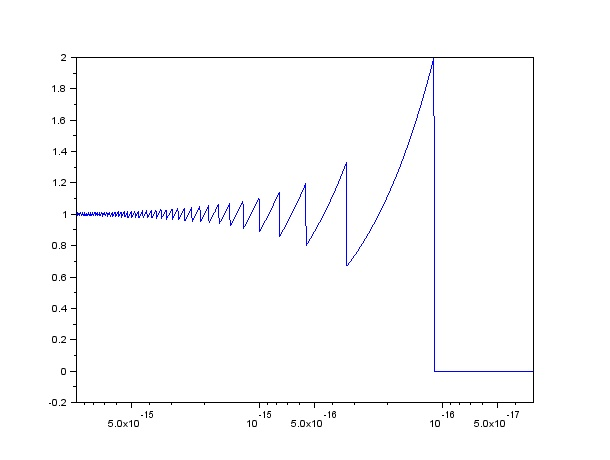
\includegraphics[width=0.8\textwidth]{cancelamento_0}


\end{ex}
\begin{prob} Considere a expressão
$$
f(x)=\frac{1-\cos(x)}{x^2}
$$
para $x$ pequeno. Verifique que
$$
\lim_{x\to 0}f(x)=0,5
$$
Depois calcule no scilab $f(x)$ para $x=10^{-5}$, $x=10^{-6}$, $x=10^{-7}$, $x=10^{-8}$, $x=10^{-9}$ e $x=10^{-10}$. Finalmente, faça uma aproximação analítica que elimine o efeito catastrófico.
\end{prob}

\begin{ex} Neste exemplo, estamos interessados em compreender mais detalhadamente o comportamento da expressão
\begin{equation}\label{def_lim}\left(1+\frac{1}{n}\right)^n\end{equation}
quando $n$ é um número grande ao computá-la em sistemas de numeral de ponto flutuante com acurácia finita.
Um resultado bem conhecido do cálculo nos diz que o limite de (\ref{def_lim}) quando $n$ tende a infinito é o número de Euler:
\begin{equation}\label{lim}\lim_{n\to \infty}\left(1+\frac{1}{n}\right)^n=e= 2,718281828459...\end{equation}

Sabemos também que a sequência produzida por (\ref{def_lim}) é crescente, isto é:
$$\left(1+\frac{1}{1}\right)^1< \left(1+\frac{1}{2}\right)^2< \left(1+\frac{1}{3}\right)^3 < \cdots $$

No entanto, quando calculamos essa expressão no Scilab, nos defrontamos com o seguinte resultado:
$$\begin{array}{|c|c|c|c|c|}
\hline &&&&\\[-0.3cm]
n & \left(1+\frac{1}{n}\right)^n&~~~~&n & \left(1+\frac{1}{n}\right)^n\\
 &&&&\\[-0.3cm]
\hline\\[-0.3cm]
1 & 2.0000000000000 && 10^{2} & 2.7048138294215 \\
2 & 2.2500000000000 && 10^{4} & 2.7181459268249 \\
3 & 2.3703703703704 && 10^{6} & 2.7182804690957 \\
4 & 2.4414062500000 && 10^{8} & 2.7182817983391 \\
5 & 2.4883200000000 && 10^{10} & 2.7182820532348 \\
6 & 2.5216263717421 && 10^{12} & 2.7185234960372 \\
7 & 2.5464996970407 && 10^{14} & 2.7161100340870 \\
8 & 2.5657845139503 && 10^{16} & 1.0000000000000 \\
9 & 2.5811747917132 && 10^{18} & 1.0000000000000 \\
10 & 2.5937424601000 && 10^{20} & 1.0000000000000 \\
\hline
\end{array}
$$
Podemos resumir esses dados no seguinte gráfico de $\left(1+\frac{1}{n}\right)^n$ em função de $n$:

%\begin{figure}[htp]
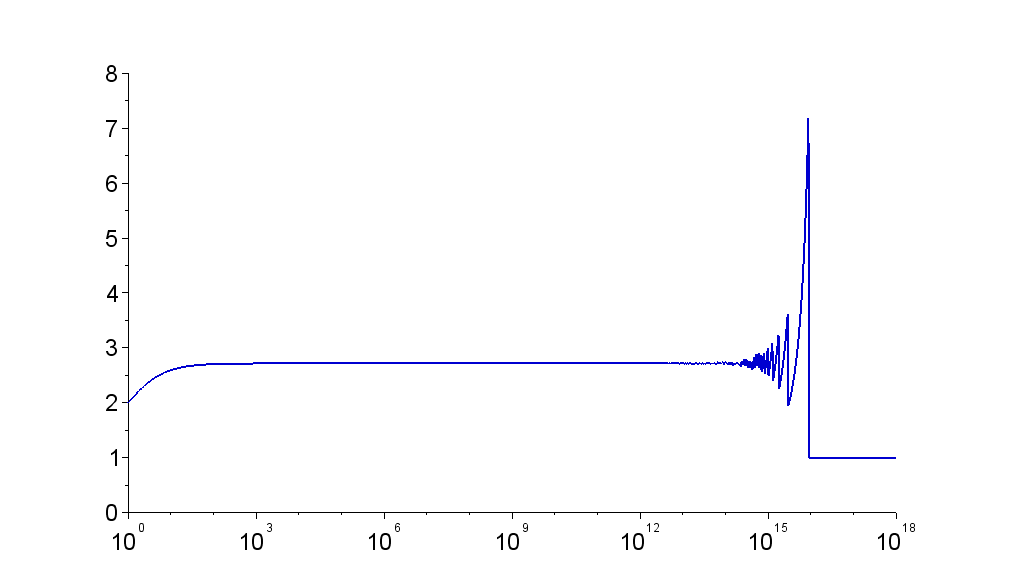
\includegraphics[width=0.8\textwidth]{cancelamento_euler}
%\caption{Gráfico de $\left(1+\frac{1}{n}\right)^n$ em função de $n$ em escala linear-logarítmica variando de $10^0$ até $10^{18}$ gerado no Scilab 5.4.1.}
%\end{figure}

Observe que quando $x$ se torna grande, da ordem de $10^{15}$, o gráfico da função deixa de se crescente e apresenta oscilações.  Observe também que a expressão se torna identicamente igual a $1$ depois de um certo limiar. Tais fenômenos não são intrínsecos da função $f(x)=(1+1/x)^x$, mas \emph{\uline{oriundas de erros de arredondamento}}, isto é, são resultados numéricos espúrios. A fim de pôr o comportamento numérico de tal expressão, apresentamos abaixo o gráfico da mesma função, porém restrito à região entre $10^{14}$ e $10^{16}$.

%\begin{figure}
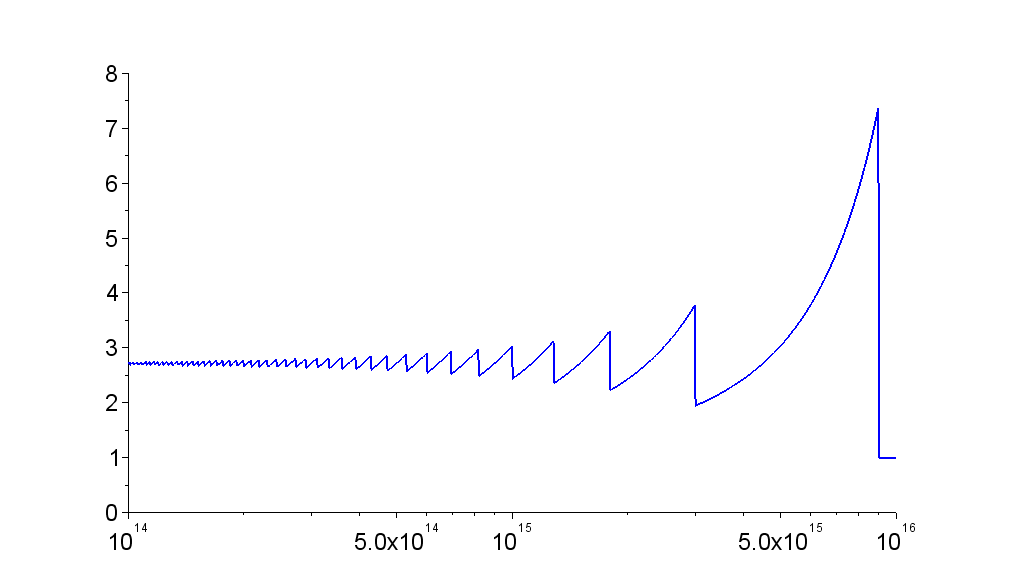
\includegraphics[width=0.9\textwidth]{cancelamento_euler2}
%\caption{Gráfico de $\left(1+\frac{1}{n}\right)^n$ em função de $n$ em escala linear-logarítmica variando de $10^{14}$ até $10^{16}$ gerado no Scilab 5.4.1.}
¨%\end{figure}


Para compreender por que existe um limiar $N$ que, quando atingido torna a expressão identicamente igual a $1$, observe a sequência de operações realizadas pelo computador:
\begin{equation}\label{seq_oper}x~\longrightarrow~ 1/x ~\longrightarrow~ 1+1/x ~\longrightarrow~ (1+1/x)^x\end{equation}
Devido ao limite de precisão da representão de números em ponto flutuante, existe um menor número representável que é maior do que 1. Este número pode ser obtido pelo comando 1+\%eps:
$$1.0000000000000002220446$$
A quantidade dada por \%eps é chamada de 'épsilon de máquina' e é o menor número que somado a 1 produz um resultado superior a 1 no sistema de numeração usado. O épsilon de máquina no sistema de numeração 'double' vale aproximadamente $2.22\times 10^{-16}$.
Quando somamos a $1$ um número positivo inferior ao épsilon de máquina, obtemos o número 1. Dessa forma, o resultado obtido pela operação de ponto flutuante $1+x$ para $0<x<2.22 \times 10^{-16}$ é 1. 

Portanto, quando realizamos a sequência de operações dada em (\ref{seq_oper}), toda informação contida no número 'x' é perdida na soma com 1 quando $1/x$ é menor que o épsilon de máquina, o que ocorre quando $x>5\times 10^{15}$. Assim $(1+1/x)$ é aproximado para '1' e a última operação se resume a '$1^x$', o que é igual a 1 mesmo quando x é grande.

Um erro comum é acreditar que o perda de significância se deve ao fato de $1/x$ ser muito pequeno para ser representado e é aproximando para $0$. Isto é falso, o sistema de ponto de flutuante permite representar números de magnitude muito inferior ao épsilon de máquina. O problema surge da limitação no tamanho da mantissa. Observe como a seguinte sequência de operações não perde significância para números positivos x muito menores que o épsilon de máquina:
\begin{equation}\label{seq_oper2}x~\longrightarrow~ 1/x ~\longrightarrow~ 1/(1/x) \end{equation}
 
compare o desempenho numérico desta sequência de operações para valores pequenos de $x$ com o da seguinte sequência:
\begin{equation}\label{seq_oper3}x~\longrightarrow~ 1+x ~\longrightarrow~ (1+x)-1 .\end{equation}

Finalmente, notamos que quando tentamos calcular $\left(1+\frac{1}{n}\right)^n$ para $n$ grande, existe perda de significância no cálculo de $1+1/n$. Para entender isso, observe o que acontece quando $n=7\times 10^{13}$:
\begin{verbatim}
-->n=7e13
 n  =
     7.000000000000000000D+13  
 
-->1/n
 ans  =
     1.428571428571428435D-14  
 
-->y=1+1/n
 y  =
 
    1.000000000000014211D+00  
\end{verbatim}
Observe a perda de informação ao deslocar a mantissa de '1/n'. Para evidenciar o fenômenos, observamos o que acontece quando tentamos recalcular n subtraindo 1 de $1+1/n$ e invertendo o resultado:
\begin{verbatim}
-->y-1
 ans  =
     1.421085471520200372D-14  
 
-->1/(y-1)
 ans  =
     7.036874417766400000D+13  
\end{verbatim}

\end{ex}

\begin{ex}[Analogia da balança] Observe a seguinte comparação interessante que pode ser feita para ilustrar os sistemas de numeração com ponto fixo e flutuante: o sistema de ponto fixo é como uma balança cujas marcas estão igualmente espaçadas; o sistema de ponto flutuante é como uma balança cuja distância entre as marcas é proporcional à massa medida. Assim, podemos ter uma balança de ponto fixo cujas marcas estão sempre distanciadas de 100g (100g, 200g, 300g, ..., 1Kg, 1,1Kg,...) e outra balança de ponto flutuante cujas marcas estão distanciadas sempre de aproximadamente um décimo do valor lido (100g, 110g, 121g, 133g, ..., 1Kg, 1,1Kg, 1,21Kg, ...) A balança de ponto fixo apresenta uma resolução baixa para pequenas medidas, porém uma resolução alta para grandes medidas. A balança de ponto flutuante distribui a resolução de forma proporcional ao longo da escala.    

Seguindo nesta analogia, o fenômeno de perda de significancia pode ser interpretado como a seguir: imagine que você deseje obter o peso de um gato (aproximadamente 4Kg). Dois processos estão disponíveis: colocar o gato diretamente na balança ou medir seu peso com o gato e, depois, sem o gato. Na balança de ponto flutuante, a incerteza associada na medida do peso do gato (sozinho) é aproximadamente 10\% de 4Kg, isto é, 400g. Já a incerteza associada à medida da uma pessoa (aproximadamente 70Kg) com o gato é de 10\% do peso total, isto é, aproximadamente 7Kg. Esta incerteza é da mesma ordem de grandeza da medida a ser realizada, tornado o processo impossível de ser realizado, já que teríamos uma incerteza da ordem de 14Kg (devido à dupla medição) sobre uma grandeza de 4Kg.    
\end{ex}